     \documentclass{beamer}
%
% Choose how your presentation looks.
%
% For more themes, color themes and font themes, see:
% http://deic.uab.es/~iblanes/beamer_gallery/index_by_theme.html
%
\mode<presentation>
{
  \usetheme{default}      % or try Darmstadt, Madrid, Warsaw, ...
  \usecolortheme{default} % or try albatross, beaver, crane, ...
  \usefonttheme{default}  % or try serif, structurebold, ...
  \setbeamertemplate{navigation symbols}{}
  \setbeamertemplate{caption}[numbered]
} 
\usepackage{amsmath}
\usepackage{amssymb}
\usepackage[english]{babel}
\usepackage[utf8x]{inputenc}


\begin{document}


% Uncomment these lines for an automatically generated outline.
%\begin{frame}{Outline}
%  \tableofcontents
%\end{frame}

\section{}

\begin{frame}{}

\begin{equation}
\dfrac{\partial u}{\partial t} = \alpha \triangledown^2 u + S
\end{equation}

u(0,y,z,t)=u(L,y,z,t)=0 \\
u(x,0,z,t)=u(x,L,z,t)=0 \\
u(x,y,0,t)=u(x,y,L,t)=0 \\

u(x,y,z,0)=f(x,y,z)


\begin{equation}
u(x,y,z,t) = \sum_{n}^{\infty}\sum_{m}^{\infty}\sum_{p}^{\infty} A_{nmp}sin(\tfrac{n\pi x}{L})sin(\tfrac{m\pi y}{L})sin(\tfrac{p\pi z}{L})e^{-\pi^2 \lambda^2 t}
\end{equation}

This is a Sturm-Liouville problem

i.e. O.D.Es of type

\begin{equation}
(P(x)y')'+(q(x)+\lambda r(x))y = 0
\end{equation}

\begin{equation}
A_{nmp}=\dfrac{(f,y_n)}{(y_n,y_n)}
\end{equation}

\vskip 1cm

\end{frame}
\begin{frame}

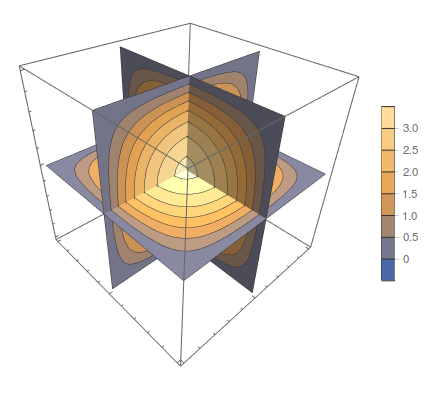
\includegraphics[scale=0.25]{analytic.png}
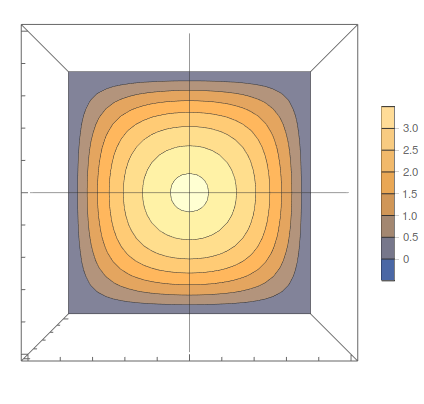
\includegraphics[scale=0.25]{top-down-analytic.png}
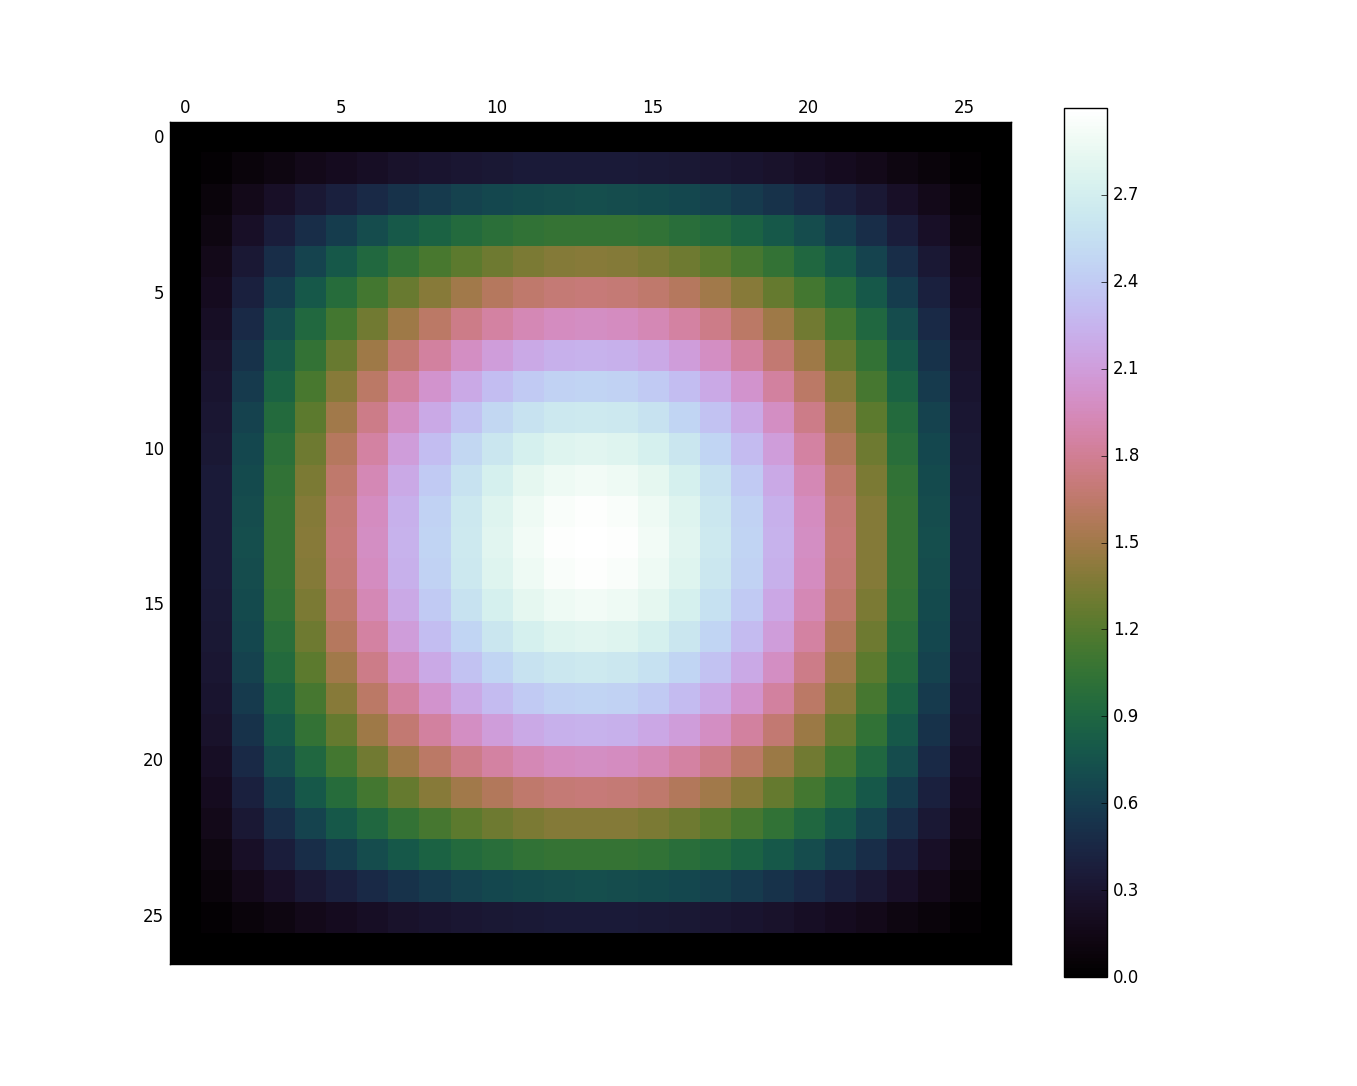
\includegraphics[scale=0.14]{numerical-sol.png}

\end{frame}

\begin{frame}
Problem:\\
Code takes ages to run for large $N>50$ \\
MC code runs on grid of $N=200ish$
\begin{figure}
\centering
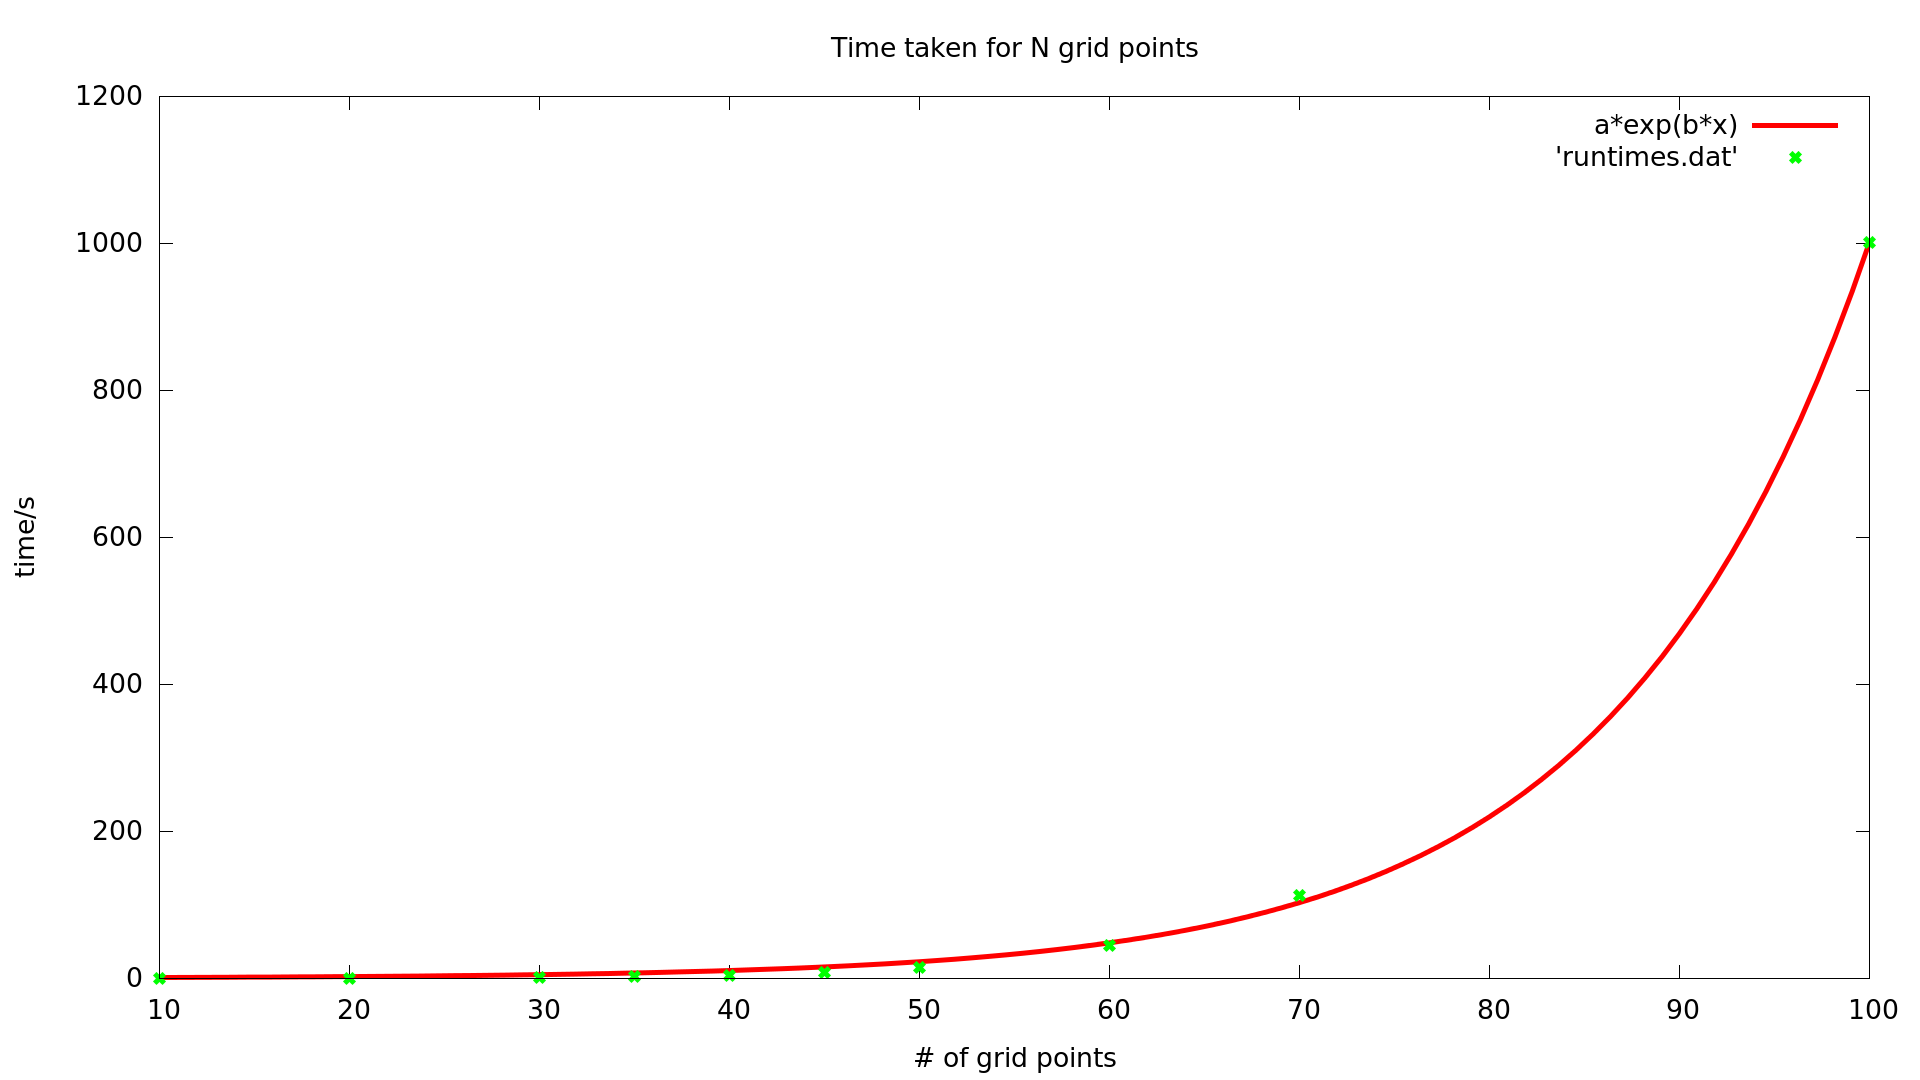
\includegraphics[scale=.17]{time.png}

\end{figure}
\end{frame}

\begin{frame}
Solution:\\
Shrink grid $=>$ Lose resolution cant model small elements
Parallelize $=>$ Not as straight forward as parallelizing MC code


\begin{equation}
\Omega(t) = \int_{t_0}^{t_f} A e^{(- \tfrac{\Delta E}{RT}) dT}
\end{equation}

%\includegraphics[scale=0.2]{high.png}
\hskip 1cm
%\includegraphics[scale=0.2]{low.png}
\end{frame}

\end{document}